

\documentclass[conference]{IEEEtran}

\usepackage{graphicx,color}
\ifCLASSINFOpdf
  % \usepackage[pdftex]{graphicx}
  % declare the path(s) where your graphic files are
  % \graphicspath{{../pdf/}{../jpeg/}}
  % and their extensions so you won't have to specify these with
  % every instance of \includegraphics
  % \DeclareGraphicsExtensions{.pdf,.jpeg,.png}
\else
  % or other class option (dvipsone, dvipdf, if not using dvips). graphicx
  % will default to the driver specified in the system graphics.cfg if no
  % driver is specified.
  % \usepackage[dvips]{graphicx}
  % declare the path(s) where your graphic files are
  % \graphicspath{{../eps/}}
  % and their extensions so you won't have to specify these with
  % every instance of \includegraphics
  % \DeclareGraphicsExtensions{.eps}
\fi



% correct bad hyphenation here
\hyphenation{op-tical net-works semi-conduc-tor}


\begin{document}

\title{Planning Paths for Rats using Actor-Critic Model}


\author{Zachary DeStefano}

% make the title area
\maketitle


\begin{abstract}
For this project, I attempted to see what paths a rat would take if the Morris Water Maze contained multiple rewards of varying value. The inspiration for this project was the layout of cities and the transportation networks used to connect them. I hoped to observe if a trained rat would use paths that look similar to those transportation networks. In order to do this, I trained the rat using hippocampal place cells that learn via temporal difference learning in the actor-critic model. After training, I started the rat at random locations and recorded the paths it took to the reward centers. In the end, the paths are suboptimal thus rats should not be used for path planning. 
\end{abstract}

\IEEEpeerreviewmaketitle



\section{Introduction}

The Morris Water Maze is one where a rat is released into a pool of water and searches for a platform which will provide relief from having to swim. The platform is thus considered a reward in the brain of the rat. Due to the constant location of these platforms, it is optimal for the rat to learn this location and it is desirable for us to model this learning.\\
\\
A common model for the neuronal activity in the rat involves place cells in the hippocampus that send signals depending on the current location of the rat. The Actor-Critic Model is used to control what the optimal next move should be for the rat. \\
\\
A common problem is transporation planning is that there are multiple locations that all need to reach each other so there needs to be a minimal cost network that connects them all. I attempted to see if rat movements could give more insights into this problem. \\

\section{Related Work}

\subsection{Foraging Behavior in Rats}
Foraging behavior for rats has been commonly studied.

\subsection{DA-STDP for foraging}

There were attempts to study foraging behavior using DA-STDP. In this paper, **CITE PLOS ONE PAPER**, they modeled a rat foraging for food in an environment. In the paper there were many issues getting the model to work thus it would have proven impractical for me to do. \\
\\
In this paper, **THE ROBOT**, they model a robot's movement via DA-STDP. While they accomplish a lot in the paper, due to the lack of place cells and other deficiencies with the input, it would have proven impractical for my purposes. Tuning DA-STDP would have been very difficult and deciding on good input parameters would also have been challenging. \\

\subsection{Slime Mode Interstates}

There was work done where food was placed at the location of the 20 largest cities in the United States and then slime mold was released. The paths sketched out by the slime mold ended up being similar to the interstate highway system. This is a great example of how the aggregate of simple actions taken by a biological organism can yield useful results. My goal with the rat experiment was to see if we would get useful results taking the aggregate of the paths it takes after learning. 


\section{Experiment Design}

\subsection{Rat Movements}

For the real experiments there would be a rat moving around a circular pool. I thus had a "rat" with an x-y location moving around a circle. In my model, the rat has place cells in its hippo-campus and each of the place cells has a preferred location in the circle. Each place cell feeds into a critic cell as well as 8 actor cells. The place cell location, responses by the actor and critic cells, and final direction chosen by the rat was determined using the model specified in Foster et al **INSERT CITATION**. \\
\\
There were two important things to consider when modeling the rat's movements: how much it changes direction and what to do if it hits the wall. For simplification, I assumed that a rat "bounces off" a wall if it hits it. This means that I had $\pi$ radians to its direction of movement in order to reverse it. When doing this, it is possible that if the rat hits the wall from a certain angle and is at the right location, then it could keep bouncing forever. **INSERT PICTURE**. If the rat failed to be at a proper location after "bouncing" then I change its direction by $\frac{\pi}{2}$ radians in order to prevent this from occurring. \\
\\
The other thing to consider is how much the rat's direction is allowed to change in each time step. Here I deviated from the design in Foster **INSERT CITATION** and chose my own method. I assumed that in each time step, the rat has only three choices: continue traveling in the same direction, move slightly to the left, or move slightly to right. Traveling in the same direction means that the angle of movement stays constant. Moving slightly to the left means that the angle increases by $\frac{\pi}{4}$ radians. Moving slightly to the right means the angle decreases by $\frac{\pi}{4}$ radians. In order to determine the rat's next move, I shifted the coordinate system so that the previous angle was the positive x-direction. If the vector representing the next angle had a positive y-value then I had the rat move slightly to the left. If the vector had a negative y-value then the rat moved slightly to the right.

\subsection{Rat Training and Rewards}

In order to train the rat, I followed the procedure used in Foster **INSERT CITATION** and used many parts of the morris\_water\_maze.m code. In each trial, the rat was released in one of 4 locations and then "moved" (as described above) until it found a reward center or 250 time steps had passed, whichever came first. Once the reward center was found, the actor critic values were updated. Unlike in Foster **INSERT CITATION**, I had multiple reward centers. Initially they all gave a reward of 1.\\
\\
In order to model foraging behavior, their reward value decreased by a constant amount each time the rat reached it. The reward center was not used once the value fell below a certain threshold. The rat was trained until a certain number of trials occurred or all the rewards had been spent, whichever came first. \\
\\
In order to see if there would be an effect if we modeled the fact that cities have different populations, I also ran trials where the initial reward values were different **IMPLEMENT THIS AND SHOW FIGURES**. I took the population values and did a rescale and shift so that they fell between 0.5 and 1. 

\subsection{Reward Center Locations}
For the reward center locations, I used basic locations to start off and then used locations inspired by the cities in the United States and Europe. \\
\\
In order to have well placed cities, for my United States map, I used New York, Chicago, Los Angeles, Atlanta, and Denver. For the Europe map, I used Paris, London, Warsaw, Berlin, and Vienna. I found their latitude and longitude coordinates in signed degrees format and plotted them on a 2D plane, rescaling for the water maze. I made sure to vary which particular set of cities I chose in a given trial. 

\subsection{Rat Testing}

Once the rat was trained, I recorded the paths it takes when released back into the maze. The rat movement was exactly the same as during training except that the actor and critic values were left unchanged. The rat also started at random locations in the maze. In order to model a random location, I used polar coordinates and chose random $\theta$ and $r$ values that are within the realm of the circle and then converted the $(r,\theta)$ pair to its corresponding $(x,y)$ pair. 
**MENTION THAT RAT MIGHT NOT STOP AT REWARD CENTERS**


\section{Results}

One of the tradeoffs was that without sufficient training, the rat tends to hang around areas that are at an equal distance from the reward centers and cannot decide which direction to go in. \\
\\
FIGURES WITH THE PATH RESULTS AND LEARNED ACTOR-CRITIC VALUES\\
INCLUDE FIGURES SHOWING CUMULATIVE DISTANCE TO THE TARGET\\
\\
It can be reasonably assumed that the highest capacity highway would need to be placed where the rat's activity is the greatest. Indeed, the region with a high amount of activity is around the center of the city points. \\
\\
For figure **INSERT REF**, I used the cities of Berlin, Vienna, and Warsaw as my model for the reward center locations. During the testing phase, the rat moves toward one of the cities and also travels around the area between the cities. The interesting thing is that if you take the areas in the figure where the path lines are densest, then it could almost make a path that would make sense as travel routes between the cities. 
**MENTION DEPRECIATION METHOD USED FOR THIS ONE**

\begin{figure}
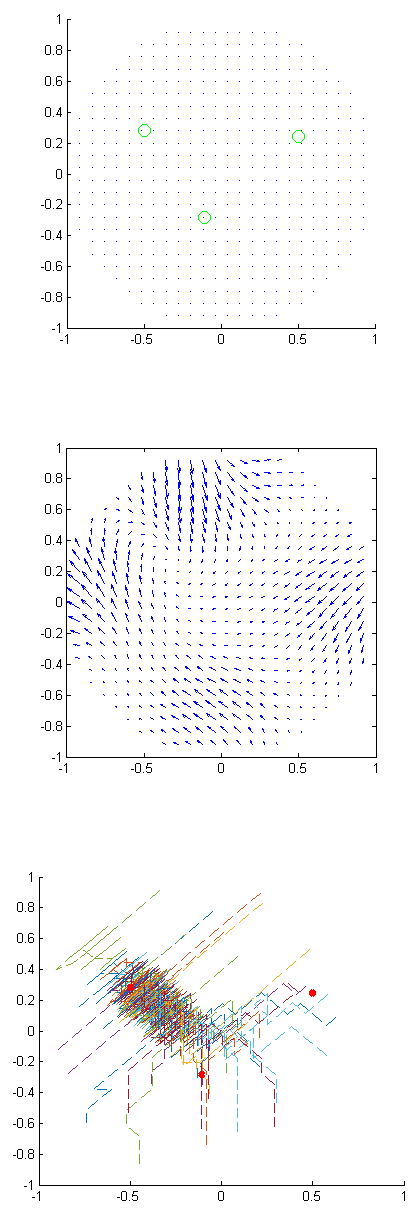
\includegraphics[width=0.4\textwidth]{waterMazeRevised2_Figure.png} 
\caption{Place Cell and Reward Center Locations (top). Actor Gradient (middle). Paths traversed by rat with reward centers in red (bottom)}
\end{figure}

\begin{figure}
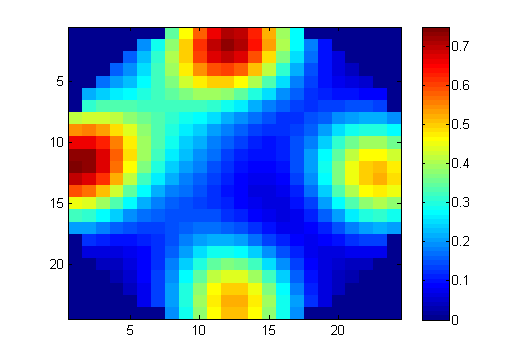
\includegraphics[width=0.4\textwidth]{waterMazeRevised2_Critic.png} 
\caption{Critic Values in Maze}
\end{figure}

For figure **INSERT REF**, I used the cities of New York, Chicago, Los Angeles, Seattle, and Atlanta. After training, the rat had relatively good actor gradient directions. When charting all the paths the rat took, there is a high density in the middle area between all the cities which would coincide with where we would want a road to be to go between all the cities. 

\begin{figure}
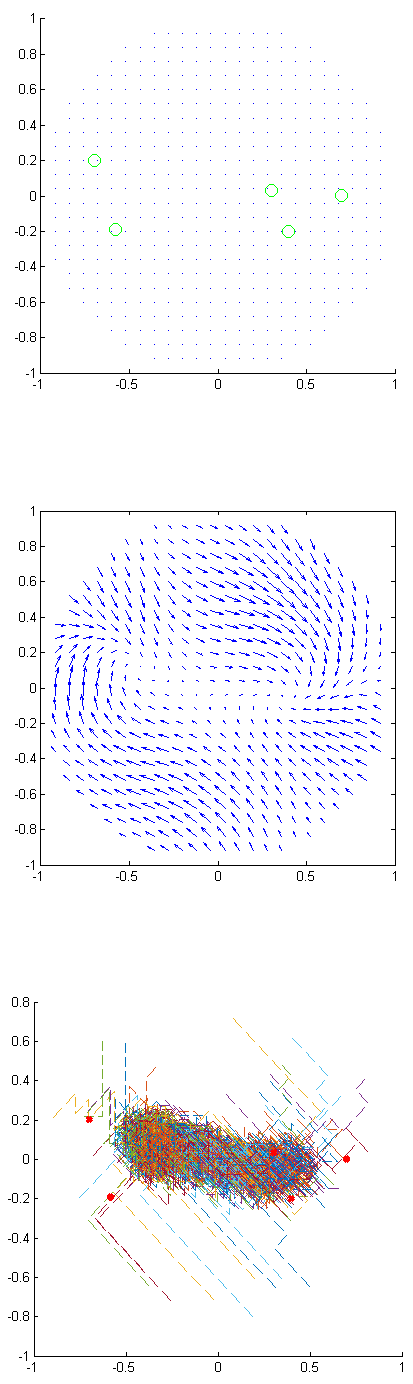
\includegraphics[width=0.4\textwidth]{waterMazeRevisedD_Figure.png} 
\caption{Place Cell and Reward Center Locations (top). Actor Gradient (middle). Paths traversed by rat with reward centers in red (bottom)}
\end{figure}

\begin{figure}
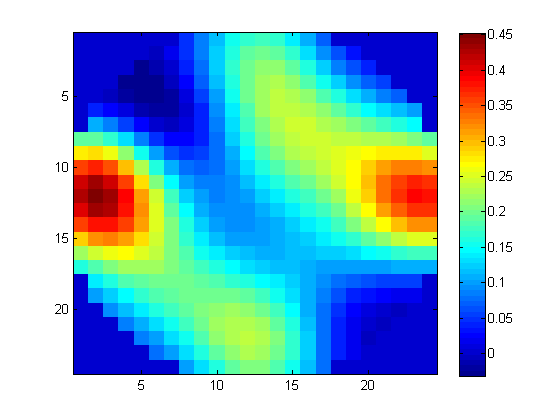
\includegraphics[width=0.4\textwidth]{waterMazeRevisedD_Critic.png} 
\caption{Critic Values in Maze}
\end{figure}

\section{Conclusion}
Rats should not be used for path planning. It was quite difficult getting the model to overcome adverse behaviors and even then, the paths taken were not terribly informative. Additionally, more efficient paths could easily be found. The hope with this project was that the actor-critic model would find compromise directions for each place cell and after enough training, you could use the actor cells to map out efficient paths all around the maze, either to the cities or between cities. 


\begin{thebibliography}{1}

\bibitem{IEEEhowto:kopka}
H.~Kopka and P.~W. Daly, \emph{A Guide to \LaTeX}, 3rd~ed.\hskip 1em plus
  0.5em minus 0.4em\relax Harlow, England: Addison-Wesley, 1999.

\end{thebibliography}




% that's all folks
\end{document}


